\chapter{Analýza}
V~této kapitole jsou popsány existující řešení úlohy detekce zboží v~ruce a~následně zmíněny zajímavé související práce týkající se termokamery. Poté je proveden rozbor zadané úlohy a stanovení nutných předpokladů pro řešitelnost. Dále jsou popsány přínosy, které termokamera v~řešení tohoto problému poskytuje a následně i překážky se kterými je nutno počítat. V~poslední části jsou představeny dostupné hardwarové a softwarové prostředky.

\section{Současný stav řešení problematiky} 
Nebyly nalezeny žádné dostupné informace o~tom, že by se problematikou zboží v~ruce zákazníka ve světě někdo zabýval. Jediné dostupné řešení lze nalézt právě u~studenta Olivera Keruľ-Kmece v~jeho bakalářské práci \cite{kerul2016detekce}, který problém řešil s~jinou technologií než se zabývá tato práce. Řešený problém je tedy stejný, ale díky rozdílnosti technologií je k~němu nutné navrhnout nové postupy a~metody.

V~jeho řešení je využita kamera Microsoft Kinect, která současně snímá klasický RGB obraz a zároveň k~tomu hloubkovou mapu. Jeho řešení využívá dva různé klasifikátory. Vstupem prvního klasifikátoru je segmentovaný záběr ruky pomocí hloubkové mapy. Na tomto vstupu se vypočítá 60 předem daných příznaků a následně je ke klasifikaci využit klasifikátor Gradient boosted trees. Druhý klasifikátor je využit ke zvýšení přesnosti algoritmu a~klasifikuje posloupnost tříd, která je získaná prvním klasifikátorem. Posloupnosti jsou rozděleny pomocí algoritmu SIFT na vložení ruky a vyjmutí ruky z~regálu.

	\subsection{Související práce s~termokamerou}
    Existuje samozřejmě velké množství prací, které se zabývají segmentací termografických snímků a detekcí objektů, ale jsou vybrány jen ty nejzajímavější, které byly nalezeny. \todo{}Nejčastěji lze nalézt práce, které se zabývají detekcí obličeje nebo detekcí gest.
    
    První z~těchto prací je \cite{saba2012dante}, která se zabývá detekcí ruky a sledování její trajektorie s~využitím termokamery a kamery Microsoft Kinect. V~uvedené práci jsou přijímány dva obrazové zdroje a to hloubková mapa a termovizní snímek. Kamery mají rozdílnou optiku, takže je nutné jednotlivé snímky perspektivně upravit. K~tomu je využita knihovna OpenCV a transformační matice homografie, která slouží pro převod mezi jednotlivými snímky. V~uvedené práci bohužel není ani zmínka o~synchronizaci kamer, která se následně v~této práci ukázala jako velký problém.
    
    V~uvedené práci je následně využito dynamického odčítání pozadí \cite{opencvMOG}, pomocí kterého je na snímcích získáno popředí. Na termovizním snímku je dále aplikováno Otsu prahování \cite{otsu1975threshold} pro získání ruky, na které jsou vypočítány konvexní body pro získání prstů. Na snímku ruky jsou pak získány atributy, které se týkají primárně teplot a snímek je klasifikován pomocí klasifikátoru SVM. 
    
    Dvě různé kamery a metoda dynamického odčítání pozadí je využita také v~práci \cite{zeng2012hand} pro detekci gest. Zarovnání dvou obrazových zdrojů je též řešeno pomocí matice homografie a synchronizace není zmíněna. Segmentace probíhá pouze formou odečtení pozadí, podle teplot se nesegmentuje. Po tomto kroku už se na snímek jen aplikují morfologické operace a následně je na snímku vyhledána ruka.
    
		Další zajímavou prací je \cite{appenrodt2010data}, kde se autor zaměřuje na detekci gest a porovnává při jednotlivé využité zdroje obrazu a to: klasický RGB, hloubkovou mapu, termovizní snímek. Následně je provedena segmentace ruky na termovizním snímku pomocí binárního prahování a tento obraz je sloučen s~nejbližšími oblastmi hloubkového obrazu. Na tomto obraze jsou dále získané atributy a snímek je klasifikován pomocí Hidden Markov Models (HMM).

Přínosná je též práce \cite{duarte2014segmentation}, kde jsou popsány běžné způsoby pro segmentaci termovizních snímků, který pak byly vyzkoušeny při řešení této práce.


Často lze objevit \cite{sato2000fast} informaci o~tom, že se počítá s~tím, že teplota ruky se pohybuje v~určitém běžném rozsahu a lze segmentovat podle teplot s~pomocí binárního prahování. Tento jednoduchý způsob se následně osvědčil i v~této práci.

\section{Analýza zadaného problému}
Zadání problému je vcelku přímočaré. Pro vstupní snímek je nutné rozhodnout, zda se na něm nachází ruka nebo ruka se zbožím a nebo se na něm nenachází nic zajímavého. Je však potřeba počítat s~tím, že se nejedná pouze o~návrh algoritmu, ale také o~získání samotných dat a v~neposlední řadě také ověření správného postupu vyhodnocením. 

Prvním nezbytným krokem je tedy zaměřit se na to, jakým způsobem budou data získávána. V~\ref{section:retrieving_camera_data} byly popsány možné metody získání dat, ze kterých plyne, že běžně dostupné softwary jsou pro tuto úlohu nedostačující. Je tedy nutné poohlédnout se po vhodném SDK, seznámit se s~jeho rozhraním a~vytvořit aplikaci pro kontinuální ukládání surových dat. Přijímaná data z~kamery není vhodné převádět do komprimovaného formátu z~důvodu zachování maximální kvality.

Dalším nutným krokem je průzkum nasnímaných dat a navržení vhodného postupu jejich předzpracování. Tento postup by měl data zejména omezit na určitou oblast zájmu a převést do normalizovaného rozsahu teplot. Podle nutnosti pak záběr patřičně upravit a nakonec redukovat šum.

Na předzpracované snímky aplikovat vhodné algoritmy a tím získat potřebné informace k~dalšímu rozhodování o~výsledku. S~přihlédnutím k~faktu, že zboží má nižší teplotu než ruka, by zboží mělo být ve většině případech rozlišitelným. Otázkou zůstává, jak velké předměty je ještě možné detekovat než je dosaženo možností algoritmu a limitu termokamery. S~limitem termokamery bude souviset generovaný šum detektoru, se kterým je nutné se vypořádat. 

Posledním krokem je klasifikace do předem definovaných tříd. Tyto třídy by mohly být tři a to: pozadí, ruka, ruka se zbožím. Vzhledem k~tomu, že určit pozadí lze triviálním způsobem, bude brána v~úvahu pouze binární klasifikace třídy ruka a ruka se zbožím.

Je zřejmé, že zboží které na~snímku není vidět, například je schované v~dlani ruky, nelze tímto způsobem detekovat. V~práci se tedy berou v~potaz pouze snímky, kde zboží viditelné je. V~práci se též neřeší o~jaký typ zboží se jedná, protože to se samotnou termokamerou není zjistitelné a~existují k~tomu lepší metody. 

\section{Nutné předpoklady}
Aby byl problém termokamerou řešitelný, musí být bráno v~potaz několik předpokladů, které souvisí s~teplotou snímaných objektů. Uvedené předpoklady pouze vylučují extrémní případy, které se běžně ve vnitřních prostředí nestávají, ale je nutné je brát na vědomí.

	\subsection{Předpoklad pro teplotu ruky na snímku}\label{section:hand_temp_prereq}
	O~termoregulaci se v~lidském těle stará část mozku s~názvem hypothalamus.  Povrchová teplota lidského těla není stabilní a v~některých situacích se znatelně mění, zato teplota lidského jádra zůstává dlouhodobě neměnná a to dokonce i v~případě velkých výkyvů okolních teplot. \cite{pvrikopa2011navrhnvete}
    
    Průměrná teplota zdravého člověka na povrchu čela je při běžných pokojových podmínkách 36 - 37 \textdegree{}C \cite{mlvcak2007mapovani}. Končetiny, a zvláště prsty, jsou vždy o~něco chladnější, protože krev nejdříve putuje přes životně důležité orgány a až poté se dostává do končetin. Rozvádění krve až do končetin je pro tělo náročné, a~v~rámci vlastních experimentálních měření bylo zjištěno, že při přechodu z~chladnějších venkovních podmínek do pokojové teploty je povrchová teplota ruky schopna klesnout i o~10 \textdegree{}C níž, než je její běžný stav. Tento pokles trvá několik minut, dokud se tělo neaklimatizuje.
    
    V~této práci se tedy počítá s~tím, že snímaný člověk se již nějakou dobu pohyboval v~běžné pokojové teplotě a teplota jeho ruky se již ustálila.
    
    \subsection{Předpoklad pro teplotu zboží a regálu na snímku}
    Regál je umístěn v~místnosti s~pokojovou teplotou a jednotlivé zboží má velmi podobnou teplotu jako je teplota vzduchu v~místnosti. Teplota zboží v~regále musí být rozlišitelná od ruky, jinak by úloha termokamerou nebyla řešitelná.
    
    \subsection{Předpoklad pro teplotu podlahy na snímku}
    Pomocí vlastních experimentálních měření bylo zjištěno,že podlaha běžné místnosti je ve většině případů o~pár desetin stupňů Celsia studenější než je teplota vzduchu v~místnosti. V~práci se počítá s~tím, že teplota podlahy nepřevyšuje teplotu zboží a tedy ani ruky na snímku.
    
\section{Výhody využití termokamery pro tuto úlohu}
Tato úloha lze samozřejmě řešit i pomocí jakékoliv barevné kamery. Například způsobem, který je uveden v~již zmíněné práci Olivera \cite{kerul2016detekce}. Všechna řešení pomocí klasické barevné kamery by k~segmentaci ruky nejčastěji využívaly její barvu. Barva kůže není přirozeně nikde definovaná a navíc je závislá na světelných podmínkách v~dané místnosti. Tento způsob segmentace tedy nemusí vždy fungovat naprosto korektně a obecně není moc dobré se na barvu kůže zcela spoléhat. Dalším možným problémem je případ, kdy má zboží podobnou barvu jako ruka, což je díky různorodosti zboží běžný případ. 

V~\ref{section:hand_temp_prereq} bylo zjištěno, že teplota ruky je silně ovlivněna působením chladného vnějšího vlivu. Tento případ je ale v~reálném světě prostředí úlohy velmi málo pravděpodobný, protože člověk se ve vnitřním prostředí často velmi rychle aklimatizuje. Pokud by přeci jen tento případ opravdu nastal a~teplota ruky klesla například z~běžných 35 \textdegree{}C na 25 \textdegree{}C, byla by stále rozlišitelná od zboží, které dosahuje pokojové teploty někde mezi 16 až 22 \textdegree{}C. Řešení s~termokamerou by tedy mělo být pro segmentaci ruky robustnější, než segmentování ruky podle barvy s~běžnou RGB kamerou.

Další výhodou je, že termokamera není závislá na světelných podmínkách. Snímá totiž pouze námi neviditelné infračervené záření (\ref{section:measurement_principle}). Z~toho plyne, že stejné výsledky lze naměřit i v~úplné tmě.

Posledním zajímavým poznatkem je, že snímání termokamery neovlivňují barvy ani vzory, takže výsledný obraz obsahuje méně rušivých elementů než například běžný RGB obraz.

\section{Překážky při snímkování s~termokamerou}
Pří snímkování s~termokamerou je nutné brát v~potaz několik skutečností, které ovlivňují snímaná data a mohou též vést k~chybným výsledkům měření. Tyto skutečnosti mohou být dané konstrukčními vlastnostmi kamery a nebo se  jedná o~uživatelské chyby nastavení.

	\subsection{Korekce signálů detektoru - NUC}\label{section:nuc}
    Tak jako běžné kamery i termokamera se při snímkování zahřívá. Změna teploty detektoru pak ovlivňuje jednotlivé mikrobolometry a to tím, že začne vznikat posun hodnot signálů (temperature drift). Tento posun zvládne kamera do určité míry kompenzovat interní logikou, ale když už posun překročí jistý limit, je automaticky spuštěna kalibrační funkce NUC neboli Non-Uniformity Correction. Termokamera vloží mezi objektiv a detektor na krátký okamžik závěrku, která simuluje jednotné homogenní prostředí. S~pomocí tohoto uniformního prostředí jsou nastaveny korekce pro normalizaci hodnot signálů. 
    
    V~době kalibrace termokamera nepřenáší obraz. Tato kalibrace trvá přibližně vteřinu a její četnost je v~závislosti na změnách teploty detektoru. Kalibraci NUC tedy může spustit i změna teploty prostředí. Z~počátku měření se NUC provádí ve velmi krátkých časových intervalech, ale jak se teplota detektoru stabilizuje, provádí se NUC již méně častěji.
    
   	Více informací o~NUC a obecně o~problému posunu signálů bolometrů se lze dočíst v~\cite{olbrycht2014new, riou2004nonuniformity}.
    
    \subsection{Přenos snímků}\label{section:transmissio_errors}
    Protokol GigE pro přenos snímku z~kamery vychází z~internetového protokolu UDP (User datagram protocol \cite{postel1980user}). To znamená, že na rozdíl od TCP (Transmission Control Protocol \cite{postel1981transmission}) protokolu odesílatel neověřuje, zda příjemce data obdržel. Může se tedy stát, že některé snímky nemusí být vůbec přijaty. Jedná se spíše o~výjimečný případ, ale přesto je potřeba s~touto skutečností počítat. 
    
  	\subsection{Vady optiky}\label{section:lens_deffects}
    Optika termokamery není, tak jako žádná optika, dokonalá. Objevují se zde optické vady stejně jako u~tradičních objektivů pro běžné kamery. Obecně lze říct, že maximální obrazovou kvalitu lze nalézt v~oblasti, která je co nejblíže středu obrazového pole. V~těchto místech je obraz nejostřejší, nezkreslený a~s~největší rozlišovací schopností. 
    
    Na obrázku \ref{fig:camera_2_lens_deffects} je zobrazen neupravený snímek neutrálního prostředí, kde je možné pozorovat optické vady termokamery FLIR A65 s~ohniskovou vzdáleností 25 mm. Z~obrázku je zřejmé, že největším problémem je vinětace v~rozích, která velmi výrazně ovlivňuje výsledné teploty v~této oblasti.
     
    \begin{figure}[h]
      \centering
      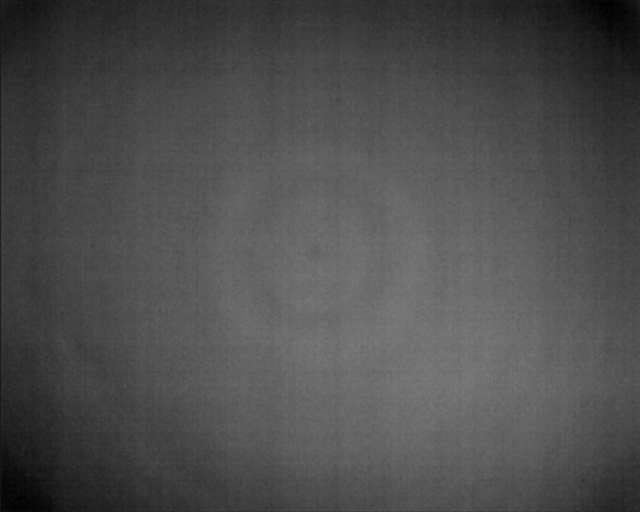
\includegraphics[width=1\textwidth]{images/camera_2_lens_deffects.jpg}
      \caption{Ukázkový snímek optických vad u~termokamery  FLIR A65 s~ohniskovou vzdáleností 25 mm}
      \label{fig:camera_2_lens_deffects}
    \end{figure}  

	\subsection{Chyby měření a vyhodnocování}
    Při snímání s~termokamerou mohou chyby vznikat už při měření a to zejména chybným nastavením kamery. Kamera na základě těchto chybných nastavení stanovuje neodpovídající teploty. Tyto parametry jsou například: emisivita, zdánlivě odražená teplota a atmosferické vlivy. V~rámci práce je nutné teploty od sebe umět rozlišit, ale není nutné znát jejich přesné hodnoty. Proto se nastavení těchto parametrů explicitně nezmiňuje a pro účely této práce nejsou klíčové. Vliv těchto parametrů a postupy, jak je správně nastavit, lze nalézt v~literatuře \cite{flirA65Spec,puhl2015bezkontaktni,smrvz2013bezkontaktni,kuvzel2010bezkontaktni}.

\section{Dostupné prostředky}
V~této části jsou popsány hardwarové a softwarové prostředky, které jsou v~rámci práce dostupné.

	\subsection{Dostupná technika}\label{sec:used_equip}
 	V~práci byly v~průběhu využity nezávisle dvě termokamery FLIR A65. Kamery se od sebe lišily ohniskovou vzdáleností a snímkovací frekvencí. Jednalo se o~kameru FLIR A65 s~ohniskovou vzdáleností 25~mm a druhou kameru stejné řady s~ohniskovou vzdáleností 13~mm. V~částech práce, kde to bude nutné, bude pro zjednodušení o~kamerách psáno už jen jako kamera (25~mm) a kamera (13~mm). Klíčové parametry těchto kamer jsou uvedeny v~tabulce \ref{table:flir_a65_spec}, všechny parametry pak lze nalézt přímo ve specifikacích výrobce \cite{flirA65Spec}.

    Využití druhé kamery bylo nezbytné, protože v~průběhu práce nastaly s~kamerou (25 mm) technické potíže a bylo nutné ji reklamovat. Aby bylo možné v~práci pokračovat, byla zajištěna náhradní kamera stejné řady, bohužel s~lehce odlišnými parametry. 
  
  \begin{table}[h]
    \centering
    \begin{tabular}{|m{5cm}|m{3.5cm}|m{3.5cm}|} \hline
      \rowcolor{Blue} \hline
      \color{White}\textbf{Specifikace} & \color{White}\textbf{Kamera (13 mm)} & \color{White}\textbf{Kamera (25 mm)} \\ \hline
      Rozlišení detektoru & \multicolumn{2}{|m{7cm}|}{ 640 $\times$ 512 pixelů } \\ \hline
      Teplotní citlivost (NETD)& \multicolumn{2}{|m{7cm}|}{< 0.05 \textdegree{}C @ +30 \textdegree{}C / 50 mK} \\ \hline
      Úhel záběru (FOV) & 45\textdegree{} $\times$ 37\textdegree{} &  25\textdegree{} $\times$  20\textdegree{} \\ \hline
      Ohnisková vzdálenost & 13 mm & 25 mm \\ \hline
      Prostorové rozlišení & 1.31 mrad & 0.68 mrad \\ \hline
      Clonové číslo & \multicolumn{2}{|m{7cm}|}{1.25} \\ \hline
      Snímkovací frekvence & 7.5 Hz & 30 Hz\\ \hline
      Zaostřování & \multicolumn{2}{|m{7cm}|}{Manuální} \\ \hline 
      Typ detektoru & \multicolumn{2}{|m{7cm}|}{Nechlazený FPA na bázi mikrobolometrů} \\ \hline
      Spektrální rozsah & \multicolumn{2}{|m{7cm}|}{7.5–13 µm, oblast LWIR} \\ \hline
      Časová konstanta detektoru & \multicolumn{2}{|m{7cm}|}{12 ms} \\ \hline
      Rozsah teplot & \multicolumn{2}{|m{7cm}|}{–25 \textdegree{}C až +135 \textdegree{}C} \\ \hline
      Přesnost měření & \multicolumn{2}{|m{7cm}|}{ $\pm$5 \textdegree{}C nebo 5 \%} \\ \hline
      Komunikační standardy & \multicolumn{2}{|m{7cm}|}{GigE vision, GenICam} \\ \hline
      Formát přenášených snímků & \multicolumn{2}{|m{7cm}|}{ 8 a 14 bit MONO Signal linear, 14 bit MONO Temperature linear} \\ \hline
      Napájení & \multicolumn{2}{|m{7cm}|}{Power over Ethernet (PoE) } \\ \hline
      Provozní teplota & \multicolumn{2}{|m{7cm}|}{–15 \textdegree{}C až +50 \textdegree{}C} \\ \hline
    \end{tabular}
    \caption{Klíčové specifikace kamer použitých v~této práci}
    \label{table:flir_a65_spec}
  \end{table}

  	Model A65 má vzhledem ke svým malým rozměrům a relativně nízké ceně nadprůměrné rozlišení. Vyšší rozlišení už se objevuje pouze u~pár modelů pro extrémní využití za mnohonásobně vyšší cenu. Další výhodou je velmi dobrá teplotní citlivost 50 mK, která je v~této třídě kamer spíše nadstandard. U~kamery (13 mm) je bohužel snímkovací frekvence velmi pomalá. 7.5 FPS je na dnešní poměry málo a pomocí této frekvence nelze běžně zaznamenávat kontinuální pohyb. Ideální by bylo, kdyby kamera (13 mm) měla minimálně 15 Hz, ale ta bohužel nebyla k~dispozici. Snímkovací frekvence kamery (25 mm) bohatě dostačuje, v~této kategorii lze též považovat za nadstandard. 
    
    Pro některé aplikace může být nevýhodou přesnost, která u~této řady nepatří mezi nejlepší. Nutno podotknout, že tato řada je primárně určená pro počítačové vidění, kde se očekává kvalitní rozlišovací schopnost (rozlišení NETD) a na přesnosti měřených teplot tolik nezáleží.

  Důležitým parametrem je také skutečnost, že kamera zvládá přenášet data v~14-bitovém Temperature linear formátu. To znamená, že jednotlivé pixely získaných nezpracovaných dat, po vynásobení konstantou, již odpovídají rovnou teplotám. Kdyby termokamera nepodporovala tento režim, ale pouze Signal linear, tak při obdržení signálu je teplotu nejprve nutno vypočíst pomocí vzorce. Více informací o~těchto dvou režimech je uvedeno v~\ref{description:transfer_data_modes}. 


  	\begin{figure}[h]
      \subfloat{{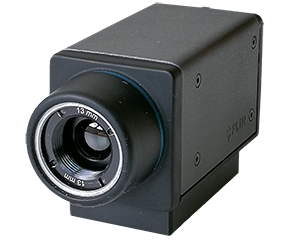
\includegraphics[width=5cm]{images/flir_a65_front.png} }}
      \qquad
      \subfloat{{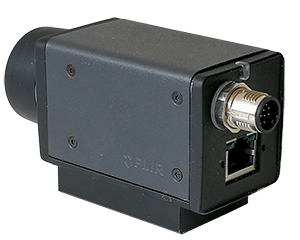
\includegraphics[width=5cm]{images/flir_a65_back.png} }}
      \caption{Termokamera FLIR A65}
      \label{fig:flir_a65}
  	\end{figure}

	\subsection{Softwarové nástroje}
    Pro získání dat z~termokamery je nutné vybrat vhodné SDK. Následně s~jeho pomocí vytvořit řídící aplikaci pro příjem dat a ovládání kamery. Ideální případ by nastal, pokud by bylo možné zvolit SDK s~rozhraním pro Javu a~integrovat jej do stejné aplikace jako navržený algoritmus.
    
    Pro algoritmus detekce bude vytvořená aplikace v~jazyce Java s~využitím knihovny OpenCV. Tato aplikace bude mít vytvořené grafické rozhraní pomocí platformy JavaFX \cite{javafx}. Grafické rozhraní ulehčí manipulaci s~daty a usnadní nastavení parametrů jednotlivých algoritmů.

Pro vyhodnocování a klasifikaci dat bude využit nástroj RapidMiner \cite{rapidminer}, který je v~tuto chvíli jeden z~nejvyužívanějších nástrojů pro data mining. Tento nástroj lze získat v~bezplatné community verzi, která má sice svá omezení, ale je pro potřeby této práce dostačující.
    
    \subsection{Volba SDK}
    Pro účely této práce by bylo nejvhodnější využít SDK ActiveGigE (\ref{section:sdk}). Poskytuje nejvíce funkcí již v~základu a je dostupné pro Javu, takže by jej bylo možné integrovat do aplikace s~detekčním algoritmem. Naneštěstí se jedná o~placené SDK a tak bylo nutné přejít k~alternativní volbě. 
    
    Jiné kompatibilní SDK, které by mělo rozhraní pro Javu neexistuje, takže bylo vybíráno na základě jednoduchosti a kvality dokumentace. Rozhodování probíhalo mezi JAI SDK a eBUS SDK, ale nakonec bylo rozhodnuto pro eBUS SDK, které je podstatně jednodušší a nabízí velké množství již implementovaných funkcionalit.
    
    \subsubsection{OpenCV}
    OpenCV \cite{opencv_library} je volně dostupná knihovna (pod licencí BSD), primárně určená pro zpracování obrazu. Je napsaná v~jazyce C/C++ a poskytuje rozhraní pro ostatní programovací jazyky jako je Java a Python. Všechny její operace jsou optimalizovány a navrhnuty pro zpracování dat v~reálném čase. Pro maximalizaci výkonu využívá hardwarové akcelerace a paralelní výpočty.